\documentclass[letter]{article}

\usepackage[english]{babel}
\usepackage[utf8]{inputenc}
\usepackage{amsmath}
\usepackage{graphicx}
\usepackage[colorinlistoftodos]{todonotes}
\usepackage{makecell}
\usepackage{multirow}
\usepackage{caption}
\usepackage{hyperref}
\usepackage[all]{hypcap}
\usepackage{enumitem}

\newlist{questions}{enumerate}{1}
\setlist[questions, 1]{label = \arabic*}
\newlist{bonus}{enumerate}{1}
\setlist[bonus, 1]{label = Bonus \arabic*}


% Adjust margins
\addtolength{\oddsidemargin}{-0.375in}
\addtolength{\evensidemargin}{-0.375in}
\addtolength{\textwidth}{1in}
\addtolength{\topmargin}{-.5in}
\addtolength{\textheight}{1.0in}

\title{CS 520: Assignment 1 - Path Planning and Search Algorithms}

\author{Haoyang Zhang, Han Wu, Shengjie Li, Zhichao Xu}

\date{\today}

\begin{document}
\maketitle

\section{Introduction, group members and division of workload}
\label{sec:Introduction}

In this group project, apart from implementing DFS, BFS, $ A^* $ with Euclidean Distance and $ A^* $ with Manhattan Distance, we also did some modification to these algorithms for different performance out of our personal interests.  \\
\begin{tabular}{| p{2.5cm} | p{11.5cm} |}
	\hline
	\makecell[c]{Name \\ RUID} & Workload \\
	\hline
	\makecell[c]{Haoyang Zhang \\ 188008687} & {Implemented DFS, Iterative Deepening DFS, BFS, Bidirectional BFS, Bidirectional $ A^* $, Beam Search, Simulated Annealing and the visualization of maze. Modified DFS to make it able to return optimal path. Added Last-in First-out feature to $ A^* $. Managed to combine Beam Search, Simulated Annealing and Genetic Algorithm. Ran tests for DFS and BFS in question 10. Finished half of the writing of report for part 2.} \\
	\hline
	\makecell[c]{Han Wu \\ 189008460} & {Wrote python scripts for testing the performance of algorithms. Combine the data and generated figures for question 1, 2, 4 and 5. Finished the writing of report for question 1, 2, 4 and 5.} \\
	\hline
	\makecell[c]{Shengjie Li \\ 188008047} & {Implemented $ A^* $ with Euclidean Distance, $ A^* $ with Manhattan Distance and Genetic Algorithm. Ran tests for $ A^* $ with Euclidean Distance and Manhattan Distance inquestion 10. Finished the format design of whole report. } \\
	\hline
	\makecell[c]{Zhichao Xu \\ 188008912} & {Wrote python scripts for testing the performance of algorithms. Combine the data and generated figures for question 3, 6 and 7. Finished the writing of report for question 3, 6 and 7. Suggested an improvement of $ A^* $ using Chebyshev Distance.} \\
	\hline
\end{tabular}


\section{Part 1: Path Planning}
\label{sec:Part 1: Path Planning}

\begin{questions}
	\item {For each of the implemented algorithms, how large the maps can be ( in terms of dim ) for the algorithm to return an answer in a reasonable amount of time (less than a minute) for a range of possible $ p $ values? Select a size so that running the algorithms multiple times will not be a huge time commitment, but that the maps are large enough to be interesting.} \\
	
	In order to find a reasonable size of the maze, we tested the running time of the algorithm. For each size, we generated 10 mazes and run different algorithms on these 10 mazes. We recorded the average time each algorithm needs to return an answer. The 10 mazes in each test ccould be either solvable or unsolvable. We set $ p $ equals to 0.3 and executed the experiment. \\
	The results are shown below as Table \ref{Table 1}:  \\
	
	\begin{center}
		\label{Table 1}
		\begin{tabular}[h]{| c | c | c | c | c | c | c | c |}
			\hline
			\multicolumn{2}{|c|}{} & \multicolumn{6}{c|}{Size} \\
			\cline{3-8}
			\multicolumn{2}{|c|}{} & 100 & 200 & 400 & 800 & 1600 & 3200 \\
			\hline
			\multirow{5}{*}{Time(s)} & DFS & 0.01942 & 0.07087 & 0.28435 & 0.93919 & 4.5064 & 10.83366 \\
			\cline{2-8}
			 & BFS\textsuperscript{2} & 0.07342 & 0.33946 & 1.73646 & 6.40967 & 25.69253 & 91.73234 \\
			 \cline{2-8}
			 & $ A^* $ Euclidean & 0.07811 & 0.41706 & 1.62604 & 5.97804 & 25.27724 & 100.37974 \\
			 \cline{2-8}
			 & $ A^* $ Manhattan & 0.06093 & 0.29222 & 0.88752 & 3.63068 & 11.147 & 63.8882 \\
			 \cline{2-8}
			 & BFS\textsuperscript{1} & \multicolumn{6}{l|}{254.36093 (size=30)} \\
			 \hline
		\end{tabular}
		\captionof{table}{}
	\end{center}

	DFS was the default setting. BFS1 was the default setting. However, it took too much time. When the size was 30, it took more than 250 seconds to return an answer. So, we changed the settings a little to make BFS acceptable. Here came BFS2. In BFS2, checkFringe=True. The others were also False. A* Euclidean means that A* algorithm used Euclidean Distance as the heuristic function. A* Euclidean means that A Star algorithm used Manhattan Distance as the heuristic function. \\
	
	In the table, we could see that when size becomes large, the average time of returning an answer (whether solvable or unsolvable) increases. BFS2 and A* Euclidean are often the most time-consuming algorithms. We need to run the algorithm repeatedly for the purpose of validations. In order to make it faster in the following test, we chose 200 as the default size of our maze. \\
	
	\item {Find a random map with $ p \approx 0.2 $ that has a path from corner to corner. Show the paths returned for each algorithm. (Showing maps as ASCII printouts with paths indicated is sufficient; however 20 bonus points are available for coding good visualizations.)} \\
	
	TODO\\
	
	\item {For a fixed value of dim as determined in Question (1), for each $ p = 0.1, 0.2, 0.3, ... , 0.9 $, generate a number of maps and try to find a path from start to goal - estimate the probability that a random map has a complete path from start to goal, for each value of $ p $. Plot your data. Note that for $ p $ close to 0, the map is nearly empty and the path is clear; for $ p $ close to 1, the map is mostly filled and there is no clear path. There is some threshhold value $ p_0 $ so that for $ p < p_0 $ , there is usually a clear path, and $ p > p_0 $ there is no path. Estimate $ p_0 $ . Which path finding algorithm is most useful here, and why?} \\
	
	In this question, we tried to use a grid-search method first to narrow down the scope of parameters. We used 200 as the mazeSize, and we generated 800 different mazes for the validation of the parameter value. \\
	
	After getting the result, we plotted the rate of successfully finding a path vs the $ p $-value. See Figure \ref{fig:3-1}. \\
	
	\begin{figure}
		\centering
		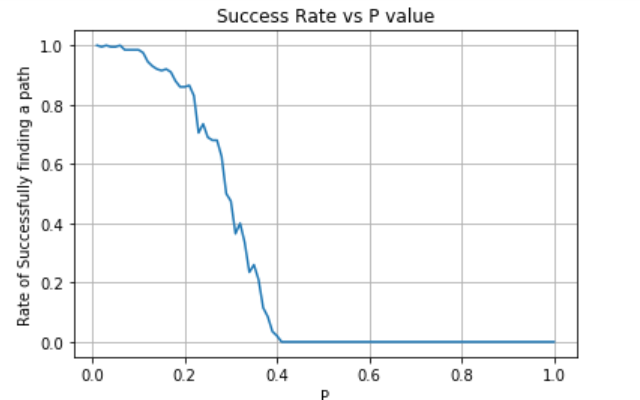
\includegraphics[width=\textwidth]{../pics/question3-1.png}
		\caption{\label{fig:3-1}rate of successfully finding a path vs the $ p $-value.}
	\end{figure}
	
	Then we tried to decrease the step size, and selected the $ p $-value from 0.16 to 0.40 as the $ x $-label to generate a new plot for better analyzing the threshold value here. See Figure \ref{fig:3-2}.\\
	
	\begin{figure}
		\centering
		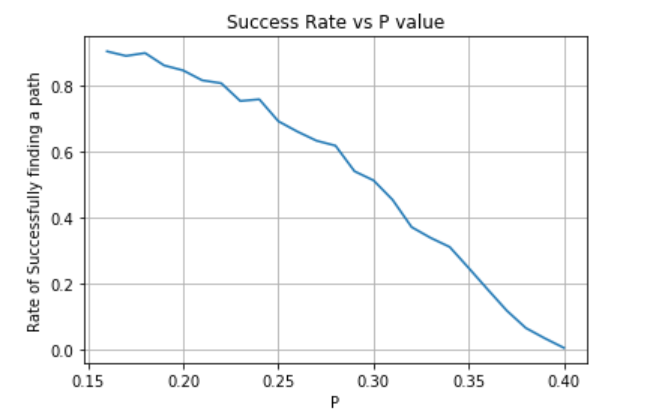
\includegraphics[width=\textwidth]{../pics/question3-2.png}
		\caption{\label{fig:3-2}rate of successfully finding a path vs the $ p $-value.}
	\end{figure}

	After analyzing the result, we notice that the when $ p $ is at 0.40, the success rate stays at 0. Thus we came to conclusion that the threshold is 0.40 for $ p $ here. And to gain a  50\%  of success rate, the $ p $-value should be set to 0.30. \\
	
	In this problem, we used the Bidirectional $ A^* $ method, and the optimal distance function is Manhattan Distance. After the calculation, we found that BD$ A^* $ consumes less time than other algorithms. In this specific problem, because we simplified the settings, we could only move to 4 directions. Manhattan Distance better simulates such scenarios thus it has the best performance here. \\
	
	
	\item {For a range of $ p $ values (up to $ p_0 $), generate a number of maps and estimate the average or expected length of the shortest path from start to goal. You may discard all maps where no path exists. Plot your data. What path finding algorithm is most useful here?} \\
	
	We set $ p $ from 0.05 to 0.35 and the step size was 0.01. For every $ p $, we generated 100 mazes and let the algorithm solve the maze. At this time, all mazes were solvable. We used $ A^* $ with Manhattan Distance to solve the problem because $ A^* $ algorithm could return the shortest path. For every $ p $, we took the average of 100 shortest path, and we plotted its relation with the probability $ p $. See Figure \ref{fig:4}: \\
		
	\begin{figure}
		\centering
		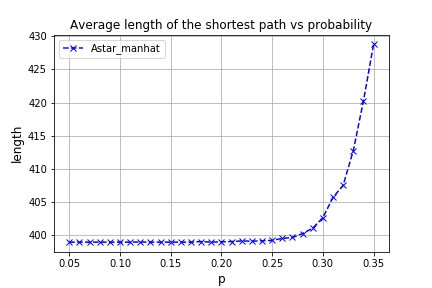
\includegraphics[width=\textwidth]{../pics/question4.png}
		\caption{\label{fig:4}rate of successfully finding a path vs the $ p $-value.}
	\end{figure}

	From Figure \ref{fig:4}, we can see that when $ p $ is less than 0.2, the average shortest is the same. Actually, it equals to the length of the shortest path from the upper left to the lower down. When $ p $ becomes greater, the average length rises fast. When $ p $ is beyond $ p_0 $, the average rises fast. \\
	
	\item {For a range of $ p $ values (up to $ p_0 $ ), estimate the average length of the path generated by $ A^* $ from start to goal (for either heuristic). Similarly, for the same $ p $ values, estimate the average length of the path generated by DFS from start to goal. How do they compare? Plot your data.} \\
	
	We generated 100 mazes under different $ p $ and used 3 algorithms -- $ A^* $ with Euclidean Distance, $ A^* $ with Manhattan Distance, and DFS(quickGoal = True, randomWalk = True) to solve the mazes. All mazes are solvable. We calculated the average path of each algorithm and plot them together. The result is shown in Figure \ref{fig:5}: \\
	
	\begin{figure}
		\centering
		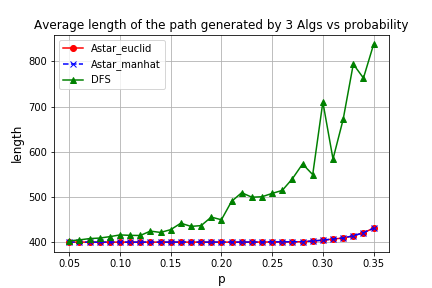
\includegraphics[width=\textwidth]{../pics/question5.png}
		\caption{\label{fig:5}rate of successfully finding a path vs the $ p $-value.}
	\end{figure}
	
	From Figure \ref{fig:5}, we can see that $ A^* $ with Euclidean Distance and $ A^* $ with Manhattan Distance have the same average shortest path. It is easy to understand this result because $ A^* $ returns the shortest path no matter what heuristic function is used. The average length of DFS is larger than $ A^* $. DFS is fast, but it can’t return the shortest path when it is not optimized. When $ p $ is greater than 0.2, the difference increases quickly. When $ p $ is large, there exists oscillation in the average length of DFS. However, we could come to conclusion that the overall trend is rising. \\
	
	
	\item {For a range of $ p $ values (up to $ p_0 $), estimate the average number of nodes expanded in total for a random map, for $ A^* $ using the Euclidean Distance as the heuristic, and using the Manhattan Distance as the heuristic. Plot your data. Which heuristic typically expands fewer nodes? Why? What about for $ p $ values above $ p_0 $?}
	
	In this question, we generated 200 different mazes to calculate our result and the mazeSize we used is 200×200 here. We used the Euclidean distance as the distance function. The result is demonstrated below as Figure \ref{fig:6-1}. \\
	
	\begin{figure}
		\centering
		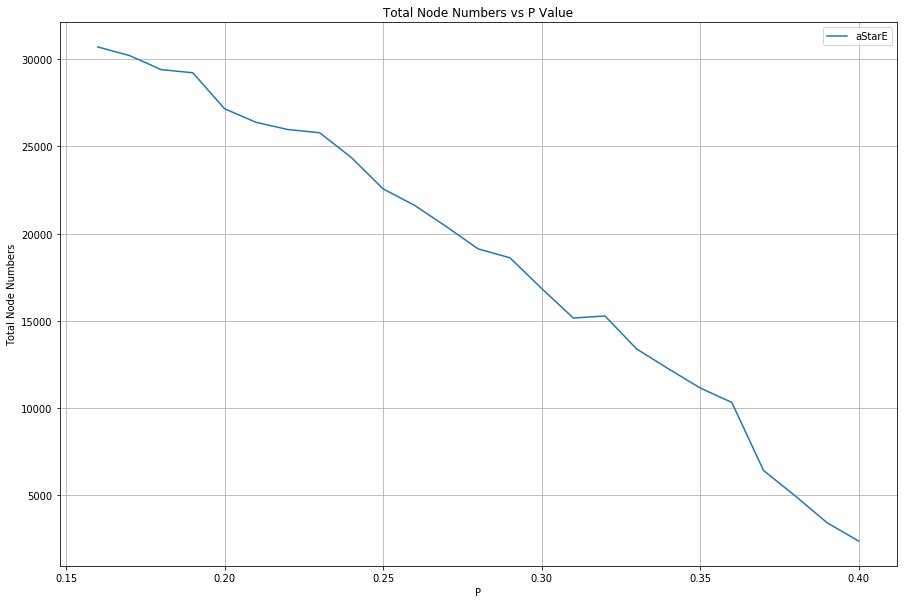
\includegraphics[width=\textwidth]{../pics/question6-1.png}
		\caption{\label{fig:6-1} $ A^* $ with Euclidean Distance.}
	\end{figure}
	
	Note that LIFO is our special bool parameter. When LIFO=True, for nodes whose heuristic values are same, the last node entering the priority queue gets popped first. \\
	
	When we used the Manhattan Distance, we conducted two tests. Figure \ref{fig:6-2} was the results of LIFO=True and Figure \ref{fig:6-3} was the results of LIFO=False. \\
	
	\begin{figure}
		\centering
		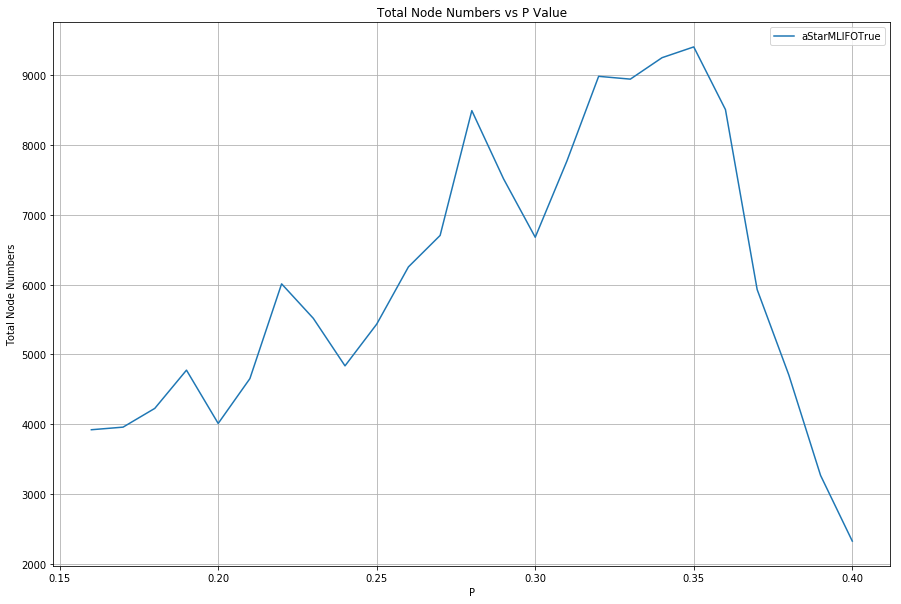
\includegraphics[width=\textwidth]{../pics/question6-2.png}
		\caption{\label{fig:6-2} $ A^* $ with Manhattan Distance when LIFO=True.}
	\end{figure}

	\begin{figure}
		\centering
		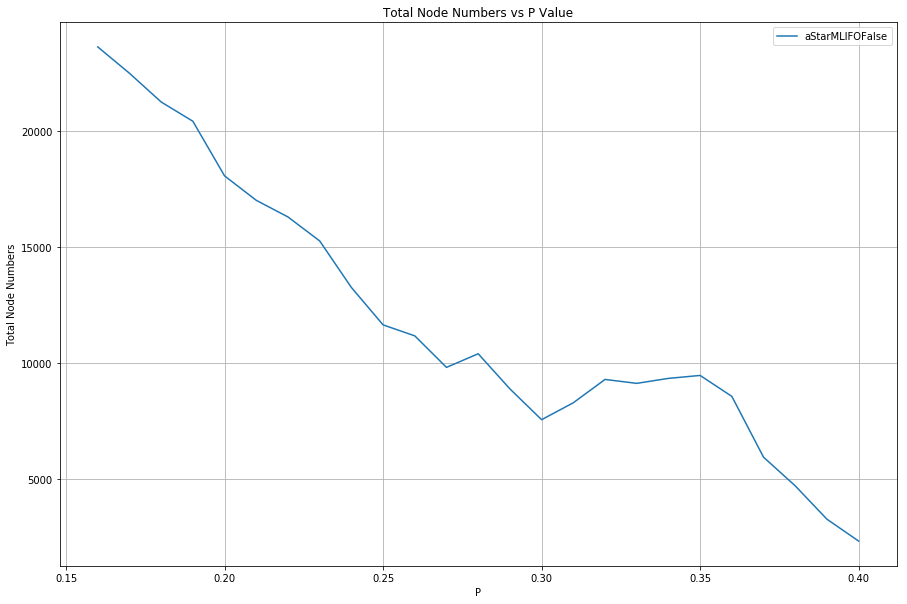
\includegraphics[width=\textwidth]{../pics/question6-3.png}
		\caption{\label{fig:6-3}$ A^* $ with Manhattan Distance when LIFO=False.}
	\end{figure}

	In this scenario, Manhattan distance when LIFO=True clearly expands fewer nodes. This is because that Manhattan is a better simulation in this scenario. We simplified the situation such that the node could only explore four directions, which suits the way M distance works. As for LIFO, when $ p $ is small enough, the whole maze almost has no walls. In this case, almost every node has the same cost thus LIFO is similar to DFS, while FIFO could be regarded as BFS. \\
	
	For the Total Node Numbers after $ p_0 $, we have Figure \ref{fig:6-4}, Figure \ref{fig:6-5} and Figure \ref{fig:6-6}: \\
	
	\begin{figure}
		\centering
		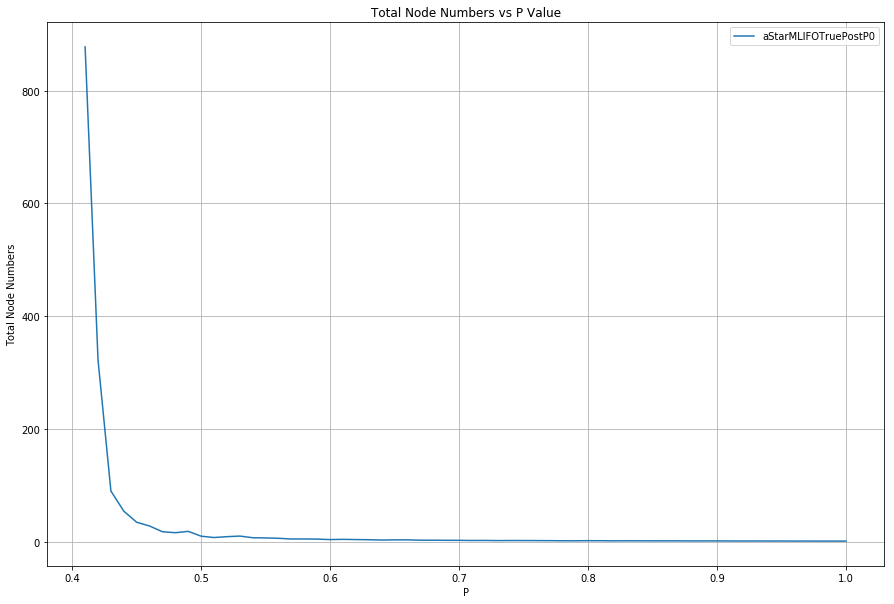
\includegraphics[width=\textwidth]{../pics/question6-4.png}
		\caption{\label{fig:6-4} $ A^* $ with Manhattan Distance when LIFO=True and $ p >= p_0 $.}
	\end{figure}
	
	\begin{figure}
		\centering
		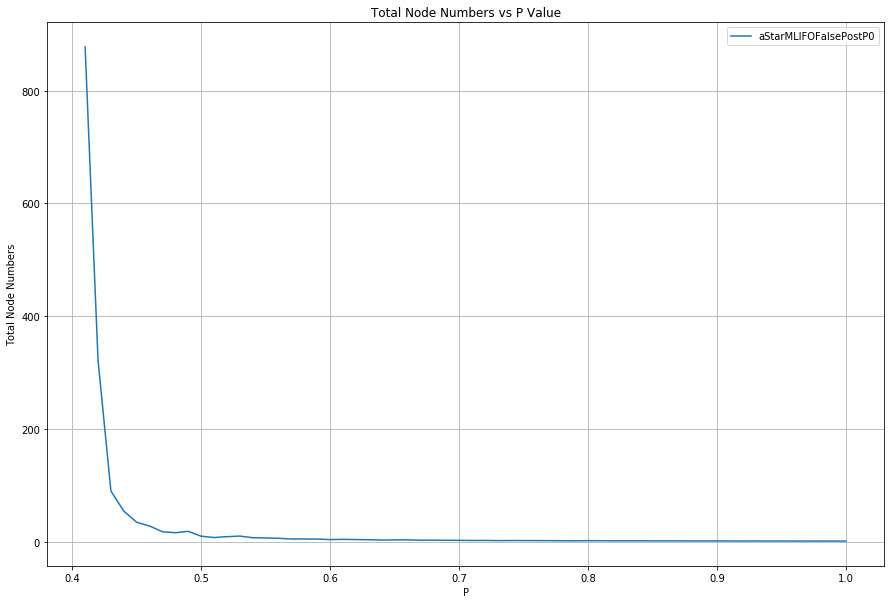
\includegraphics[width=\textwidth]{../pics/question6-5.png}
		\caption{\label{fig:6-5}$ A^* $ with Manhattan Distance when LIFO=False and $ p >= p_0 $.}
	\end{figure}

	\begin{figure}
		\centering
		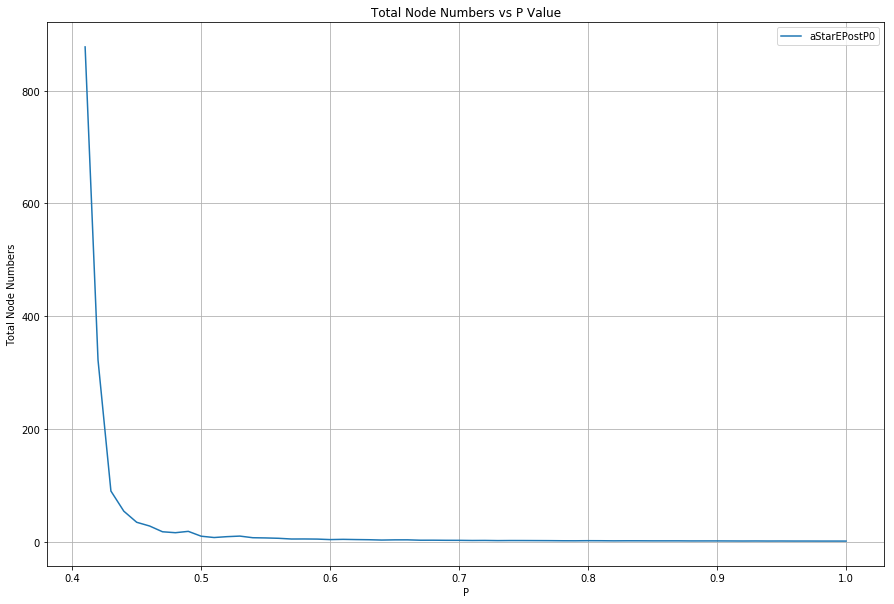
\includegraphics[width=\textwidth]{../pics/question6-6.png}
		\caption{\label{fig:6-6} $ A^* $ with Euclidean Distance when $ p >= p_0 $.}
	\end{figure}
	
	From these figures, we could tell when $ p >= p_0 $, their shape are similar. \\
	
	\item {For a range of $ p $ values (up to $ p_0 $), estimate the average number of nodes expanded in total for a random map by DFS and by BFS. Plot your data. Which algorithm typically expands fewer nodes? Why? How does either algorithm compare with $ A^* $ in Question (6)?} \\
	
	In this question, we generated 200 different mazes to calculate our result and the mazeSize we used is 200×200 here.  The result for DFS is shown as Figure \ref{fig:7-1}: \\
	
	\begin{figure}
		\centering
		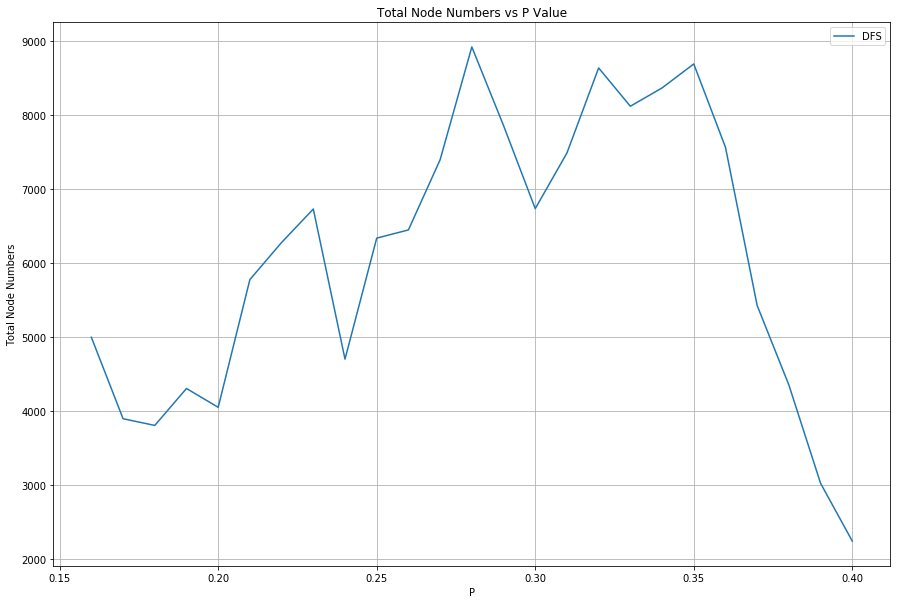
\includegraphics[width=\textwidth]{../pics/question7-1.png}
		\caption{\label{fig:7-1} Average number of nodes expanded for different $ p $ using DFS.}
	\end{figure}

	When we used the BFS, the result is shown as Figure \ref{fig:7-2}: \\
	
	\begin{figure}
		\centering
		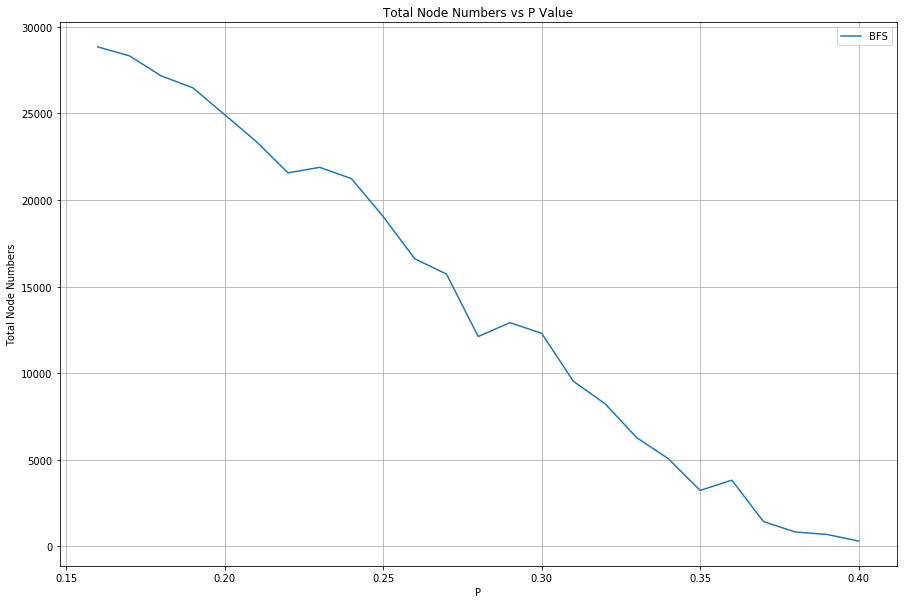
\includegraphics[width=\textwidth]{../pics/question7-2.png}
		\caption{\label{fig:7-2} Average number of nodes expanded for different $ p $ using BFS.}
	\end{figure}

	When $ p $ is low, DFS does not need to trackback for a lot of times. As $ p $ increases, DFS needs to traceback more. Such that the nodes DFS explores increases as $ p $-value grows. Also, DFS performs better than BFS. When DFS explores a path, it will go down the path until it come to a dead end. At the same time, BFS will explore all the nodes it is adjacent to. In the maze-exploration problem, the correct path often exists in the middle of the nodes, thus typically DFS overperforms BFS. \\
	
	To draw the comparison, we have Figure \ref{fig:7-3}: \\
	
	\begin{figure}
		\centering
		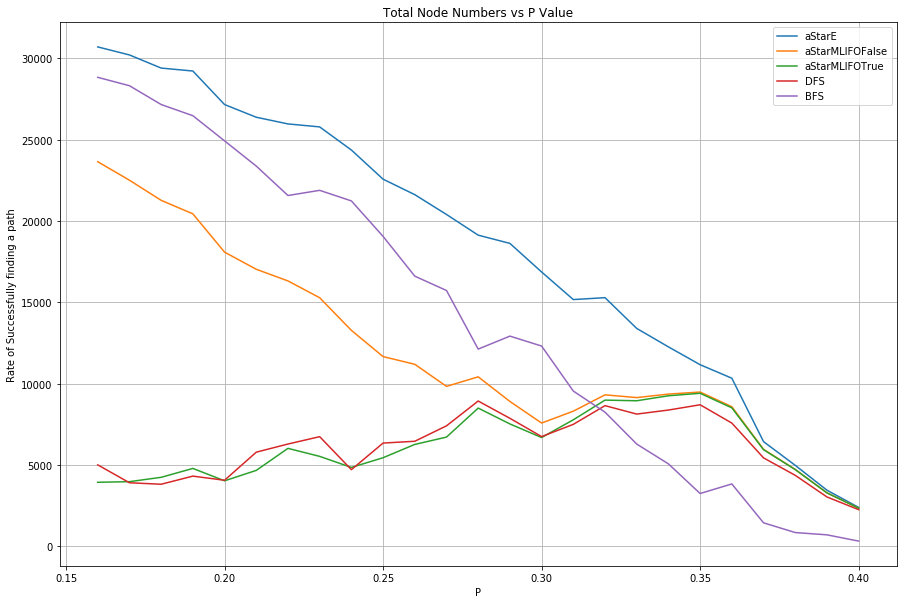
\includegraphics[width=\textwidth]{../pics/question7-3.png}
		\caption{\label{fig:7-3} Comparison of average number of nodes expanded.}
	\end{figure}
	
	
\end{questions}

\begin{bonus}
	\item {Why were you not asked to implement UFCS?} \\
	UFCS is equal to $ A^* $ algorithm with a heuristic function that always returns 0. In this mazerunner case, the cost of all steps are 1, so UFCS is exactly equal to BFS.
\end{bonus}

\section{Part 2: Building Hard Mazes}
	\label{sec:Part 2: Building Hard Mazes}
	\begin{enumerate}[resume]
		
		\item {What local search algorithm did you pick, and why? How are you representing the maze/environment, to be able to utilize your chosen search algorithm? What design choices did you have to make to apply this search algorithm to this problem?}
		
		\item {Unlike the problem of solving a maze, for which the ‘goal’ is well-defined, it is difficult to know when we have constructed the ‘hardest’ maze. That being so, what kind of termination conditions can you apply to your search algorithm to generate ‘hard’ if not the ‘hardest’ mazes? What kind of shortcomings or advantages do you anticipate your approach having?}
		
		\item {For each of the following algorithms, do the following: Using your local search algorithm, for each of the following properties indicated, generate and present three mazes that attempt to maximize the indicated property. Do you see any patterns or trends? How can you account for them? What can you hypothesize about the ‘hardest’ maze, and how close do you think you got to it?}
	\end{enumerate}
\end{document}